\documentclass{minimal}
\usepackage{graphicx,color}
\usepackage[papersize={576.00bp,432.00bp},text={576.00bp,432.00bp}]{geometry}
\begin{document}
\centering
% Title: glps_renderer figure
% Creator: GL2PS 1.3.8, (C) 1999-2012 C. Geuzaine
% For: Octave
% CreationDate: Sat Nov 11 01:53:11 2017
\setlength{\unitlength}{1pt}
\begin{picture}(0,0)
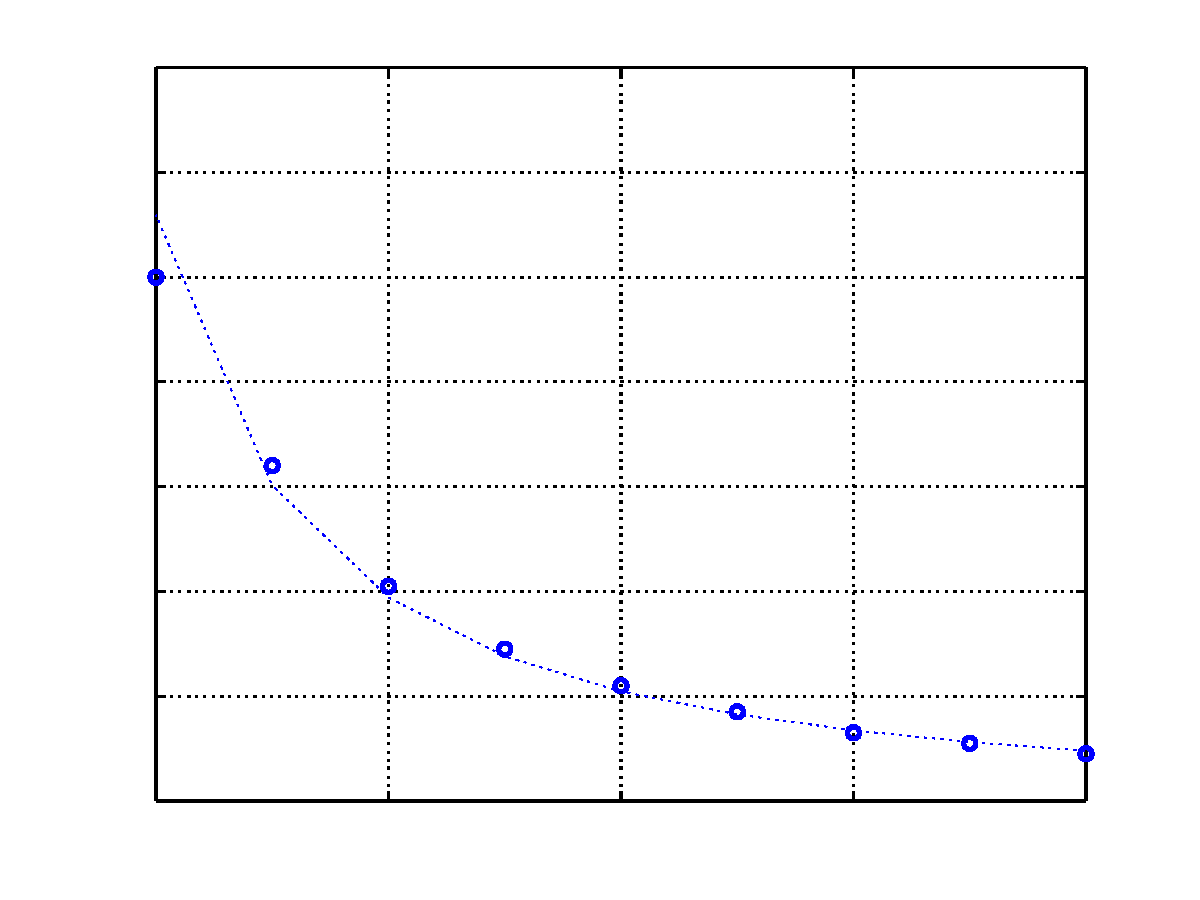
\includegraphics{illuminance_distance-inc}
\end{picture}%
\begin{picture}(576,432)(0,0)
\fontsize{12}{0}
\selectfont\put(74.88,42.5189){\makebox(0,0)[t]{\textcolor[rgb]{0,0,0}{{20}}}}
\fontsize{12}{0}
\selectfont\put(186.48,42.5189){\makebox(0,0)[t]{\textcolor[rgb]{0,0,0}{{40}}}}
\fontsize{12}{0}
\selectfont\put(298.08,42.5189){\makebox(0,0)[t]{\textcolor[rgb]{0,0,0}{{60}}}}
\fontsize{12}{0}
\selectfont\put(409.68,42.5189){\makebox(0,0)[t]{\textcolor[rgb]{0,0,0}{{80}}}}
\fontsize{12}{0}
\selectfont\put(521.28,42.5189){\makebox(0,0)[t]{\textcolor[rgb]{0,0,0}{{100}}}}
\fontsize{12}{0}
\selectfont\put(69.8755,47.52){\makebox(0,0)[r]{\textcolor[rgb]{0,0,0}{{0}}}}
\fontsize{12}{0}
\selectfont\put(69.8755,97.8171){\makebox(0,0)[r]{\textcolor[rgb]{0,0,0}{{0.2}}}}
\fontsize{12}{0}
\selectfont\put(69.8755,148.114){\makebox(0,0)[r]{\textcolor[rgb]{0,0,0}{{0.4}}}}
\fontsize{12}{0}
\selectfont\put(69.8755,198.411){\makebox(0,0)[r]{\textcolor[rgb]{0,0,0}{{0.6}}}}
\fontsize{12}{0}
\selectfont\put(69.8755,248.709){\makebox(0,0)[r]{\textcolor[rgb]{0,0,0}{{0.8}}}}
\fontsize{12}{0}
\selectfont\put(69.8755,299.006){\makebox(0,0)[r]{\textcolor[rgb]{0,0,0}{{1}}}}
\fontsize{12}{0}
\selectfont\put(69.8755,349.303){\makebox(0,0)[r]{\textcolor[rgb]{0,0,0}{{1.2}}}}
\fontsize{12}{0}
\selectfont\put(69.8755,399.6){\makebox(0,0)[r]{\textcolor[rgb]{0,0,0}{{1.4}}}}
\fontsize{16}{0}
\selectfont\put(298.08,28.5189){\makebox(0,0)[t]{\textcolor[rgb]{0,0,0}{{Distance (cm)}}}}
\fontsize{16}{0}
\selectfont\put(45.8755,223.56){\rotatebox{90}{\makebox(0,0)[b]{\textcolor[rgb]{0,0,0}{{Illuminance ratio}}}}}
\fontsize{12}{0}
\selectfont\put(136.26,223.56){\makebox(0,0)[l]{\textcolor[rgb]{0,0,0}{{F(x) = 108.313$x^{-1.52654}$}}}}
\fontsize{12}{0}
\selectfont\put(136.26,210.986){\makebox(0,0)[l]{\textcolor[rgb]{0,0,0}{{$R^2$ = 0.9761}}}}
\end{picture}
\end{document}
